
\FloatBarrier

\appendix

\begin{center}
{\LARGE{Online Appendix}}

{``Applying Data Synthesis for Longitudinal Business Data across Three Countries''}

\textit{M. Jahangir Alam, Benoit Dostie, J\"org Drechsler, Lars Vilhuber}

\end{center}


\section{Figures for the Manufacturing Sector in Canada}
\label{sec:appendix_figures}

\begin{figure}[H]
\centering
\begin{subfigure}[h]{0.48\linewidth}
\label{tab:Can:GrossEmploymentPrivate}
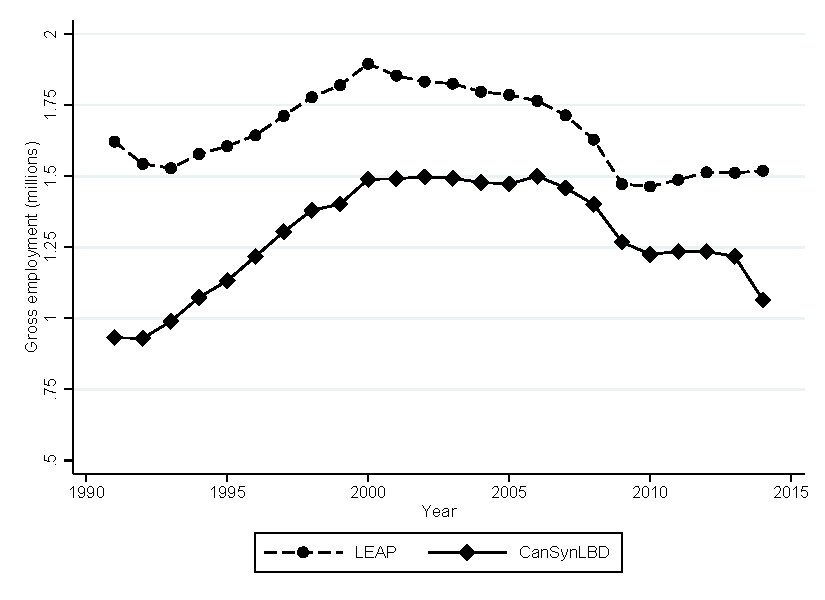
\includegraphics[width=\linewidth]{graphs/Gross_employment_level_by_year_manufacturing_bw.pdf} 
\caption{Gross employment level by year} %\begin{minipage}{0.85\textwidth}
%{\footnotesize Note: \CanTableNote \par}
%\end{minipage}
\end{subfigure}
\hfill
\begin{subfigure}[h]{0.48\linewidth}
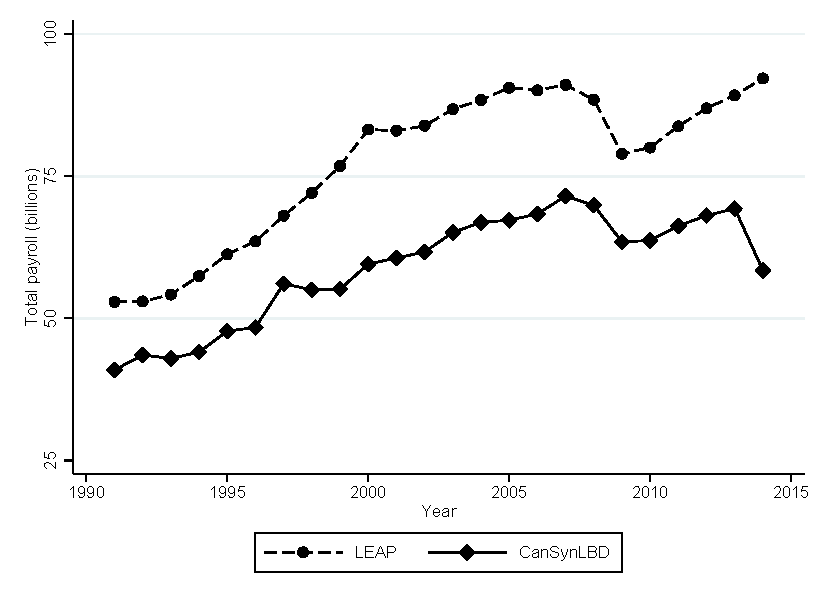
\includegraphics[width=\linewidth]{graphs/Total_payroll_by_year_manufacturing_bw.pdf}
\caption{Total payroll}
\end{subfigure}%
\caption{Entity characteristics for the manufacturing sector in Canada by year.}\label{fig:entity_chracteristics_manufac}
\end{figure}


\begin{figure}[H]
\begin{subfigure}[h]{0.48\linewidth}
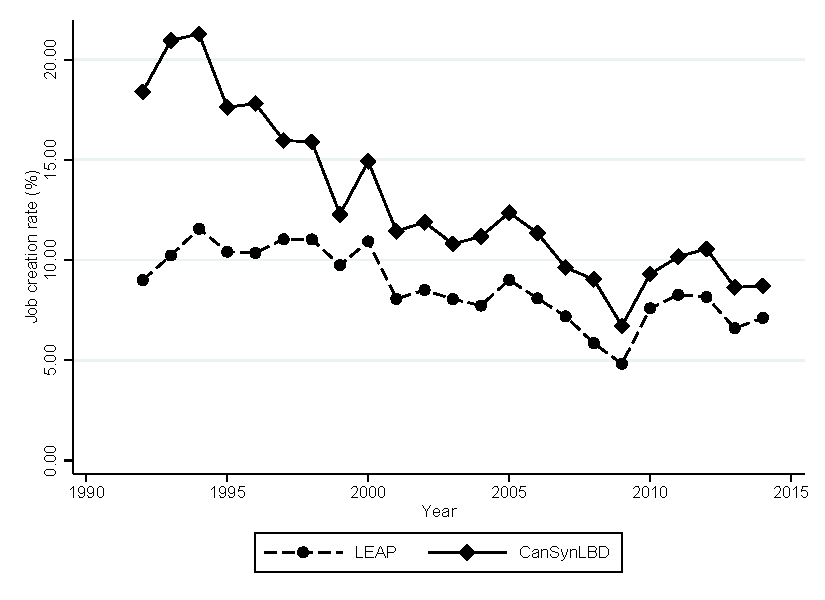
\includegraphics[width=\linewidth]{graphs/Job_creation_rate_by_year_Manufacturing_bw.pdf}
\caption{Job creation rates}
\end{subfigure}
\hfill
\begin{subfigure}[h]{0.48\linewidth}
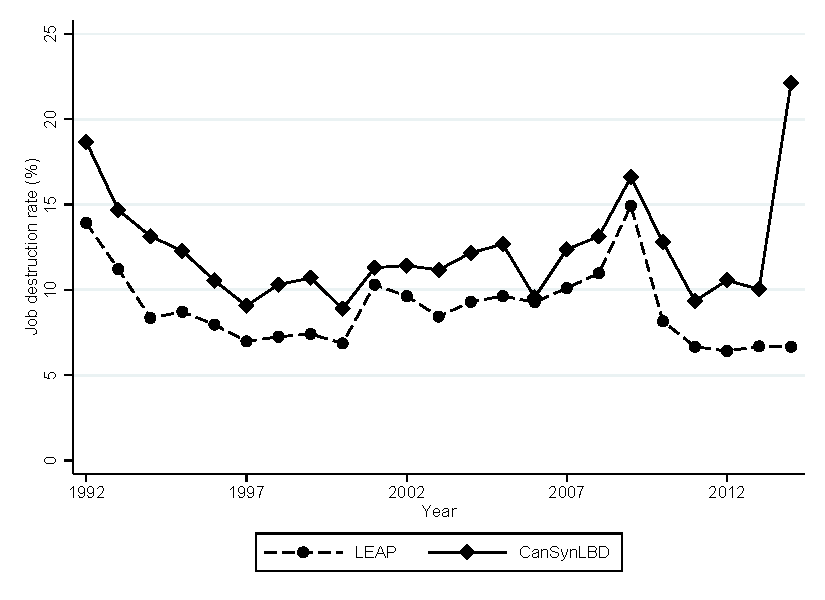
\includegraphics[width=\linewidth]{graphs/Job_destruction_rate_by_year_Manufacturing_bw.pdf}
\caption{Job destruction rates}
\end{subfigure}%
\caption{Dynamics of job flows for the manufacturing sector in Canada by year.}\label{fig:job_flows_manufac}
\end{figure}



%\begin{figure} [H]
%\centering
%\caption{Gross employment level by year (manufacturing)} %\label{tab:Can:GrossEmploymentManufacturing}
%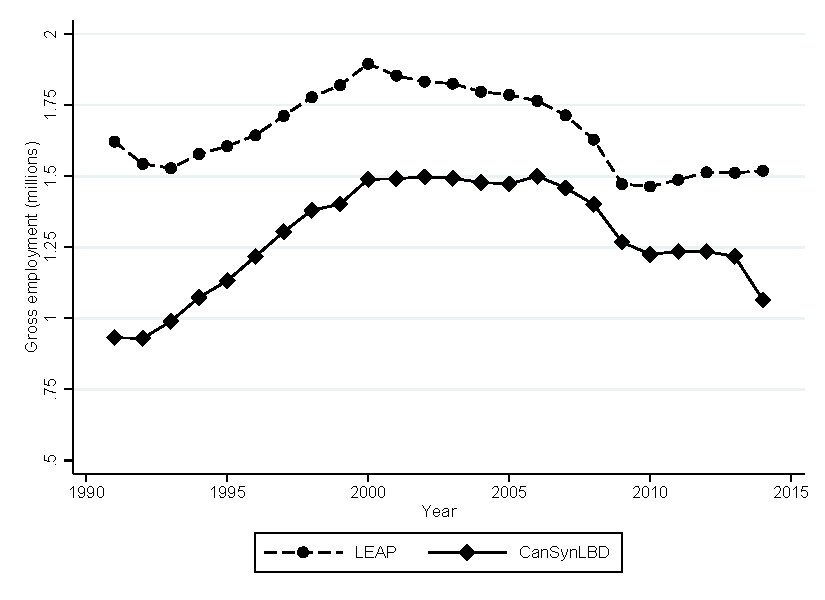
\includegraphics[height=2.8in, width=.7\linewidth]{graphs/Gross_employment_level_by_year_manufacturing_bw.pdf} 

%\begin{minipage}{0.85\textwidth}
%{\footnotesize Note: \CanTableNote  \par}
%\end{minipage}
%\end{figure}


%\begin{figure} [H]
%\centering
%\caption{Total payroll by year (private)} \label{tab:Can:TotalPayrollPrivate}
%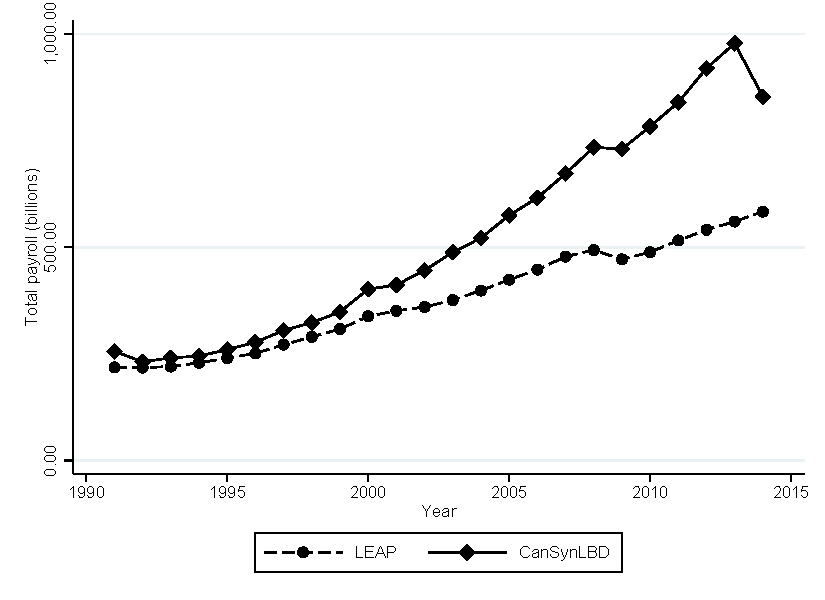
\includegraphics[height=2.8in, width=.7\linewidth]{graphs/Total_payroll_by_year_private_bw.pdf} 
%\begin{minipage}{0.85\textwidth}
%{\footnotesize Note: \CanTableNote \par}
%\end{minipage}
%\end{figure}
%\begin{figure} [H]
%\centering
%\caption{Total payroll by year (manufacturing)} \label{tab:Can:TotalPayrollManufacturing}
%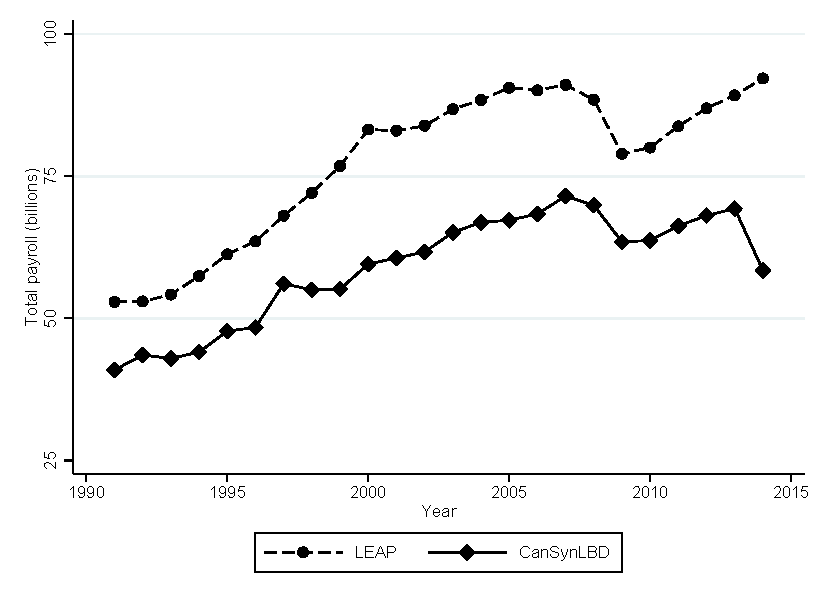
\includegraphics[height=2.8in, width=.7\linewidth]{graphs/Total_payroll_by_year_manufacturing_bw.pdf} 
%\begin{minipage}{0.85\textwidth}
%{\footnotesize Note: \CanTableNote \par}
%\end{minipage}
%\end{figure}




%\begin{figure} [H]
%\centering
%\caption{Job creation rate by year (private)} \label{JobCreationPrivate}
%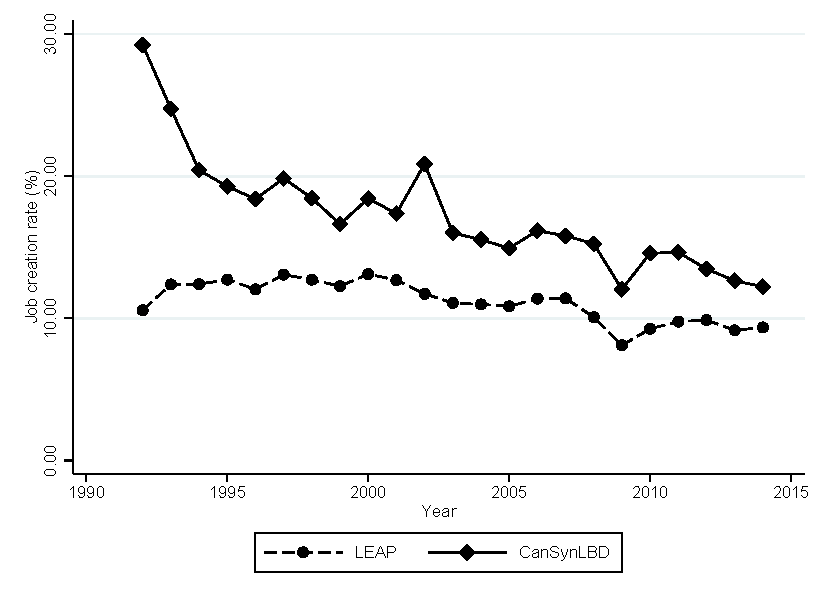
\includegraphics[height=2.8in, width=.7\linewidth]{graphs/Job_creation_rate_by_year_private_bw.pdf} 
%\begin{minipage}{0.85\textwidth}
%{\footnotesize Note: \CanTableNote \par}
%\end{minipage}
%\end{figure}

%\begin{figure} [H]
%\centering
%\caption{Job creation rate  by year (manufacturing)} %\label{JobCreationManufacturing}
%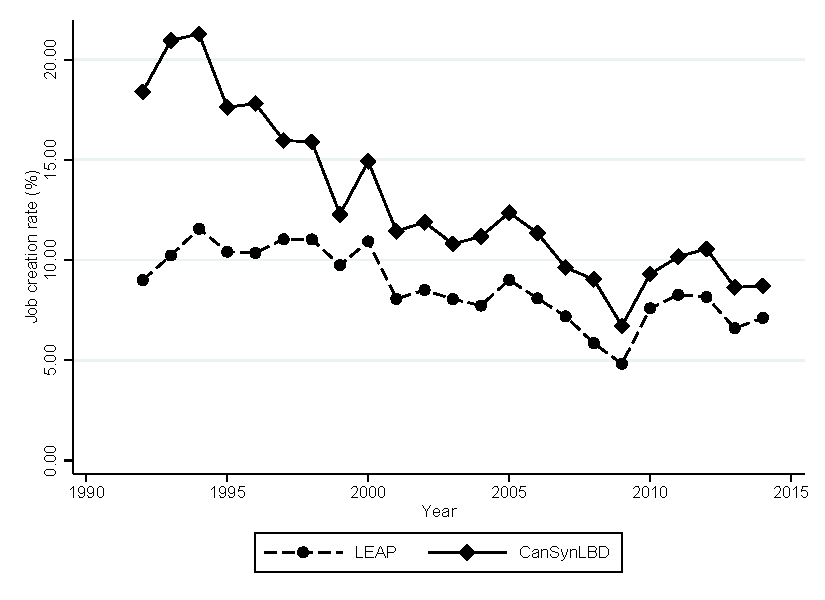
\includegraphics[height=2.8in, width=.7\linewidth]{graphs/Job_creation_rate_by_year_Manufacturing_bw.pdf} 
%\begin{minipage}{0.85\textwidth}
%{\footnotesize Note: \CanTableNote \par}
%\end{minipage}
%\end{figure}

%\todo{LV regraph, dropping last year} \todo{JA: Should we mention this in the text including reasons if we drop the last year here?}
%\begin{figure} [H]
%\centering
%\caption{Net job creation rate by year (private)} \label{NetJobCreationPrivate}
%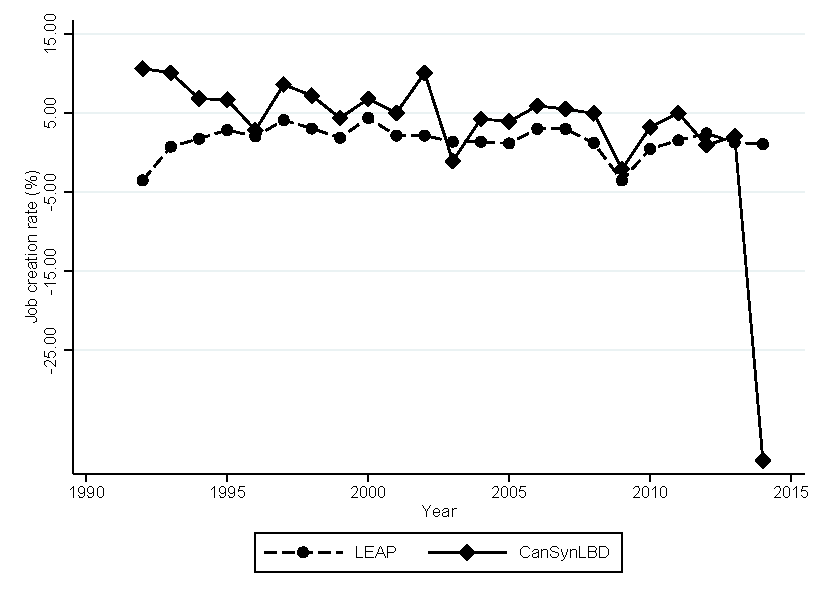
\includegraphics[height=2.8in, width=.7\linewidth]{graphs/Net_job_creation_rate_by_year_private_bw.pdf} 
%\begin{minipage}{0.85\textwidth}
%{\footnotesize Note: \CanTableNote \par}
%5\end{minipage}
%\end{figure}
%\begin{figure} [H]
%\centering
%\caption{Net job creation rate  by year (manufacturing)} \label{NetJobCreationManufacturing}
%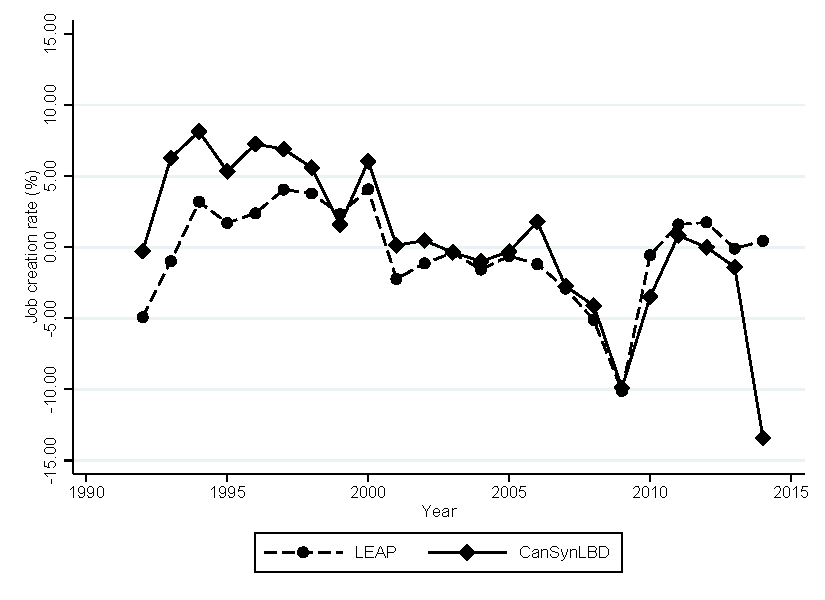
\includegraphics[height=2.8in, width=.7\linewidth]{graphs/Net_job_creation_rate_by_year_Manufacturing_bw.pdf} 
%\begin{minipage}{0.85\textwidth}
%{\footnotesize Note: $LEAP$ is the Longitudinal Employment Analysis Program and $CanSynLBD$ is the Canadian synthetic database based on LEAP. In this graph, we use 2015 vintage of LEAP for the manufacturing sector and drop last year observation of each firm. \par}
%\end{minipage}
%\end{figure}

%\todo{LV: Do we want to graph the entry/exit rates, or only the divergence?}
%\begin{figure} [H]
%\centering
%\caption{Divergence of exit and entry rate between LEAP and CanSynLBD} \label{Divergence}
%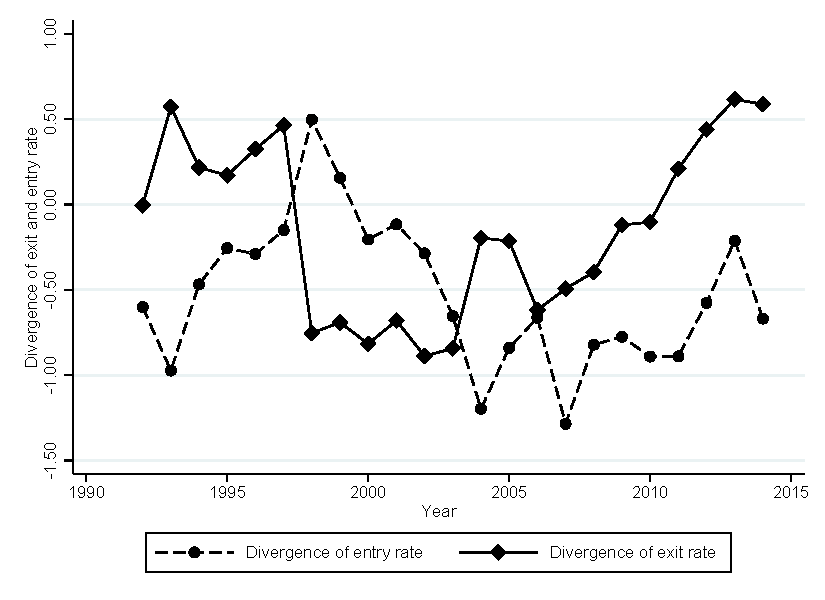
\includegraphics[height=2.8in, width=.7\linewidth]{graphs/Divergence_of_exit_and_entry_rate_between_LEAP_and_CanSynLBD_bw.pdf} 
%\begin{minipage}{0.85\textwidth}
%{\footnotesize Note: \CanTableNote  We calculate the divergence of entry rate as the entry rate of CanSynLBD net the entry rate of LEAP and the divergence of exit rate as the exit rate of CanSynLBD net the exit rate of LEAP. \par}
%\end{minipage}
%\end{figure}

\begin{figure}[H]
\centering
\begin{subfigure}[h]{0.5\linewidth}
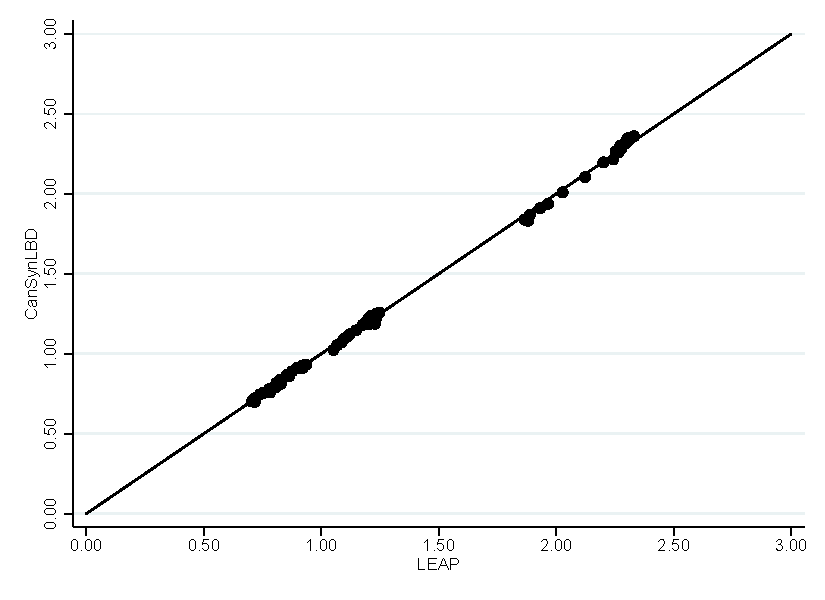
\includegraphics[trim=0 10 0 0,clip, width=\linewidth]{graphs/Share_of_firms_by_NAICS_two-digit_and_year_Manufacturing_bw.pdf}
%\caption{CanSynLBD}
\end{subfigure}\\
\begin{subfigure}[h]{0.5\linewidth}
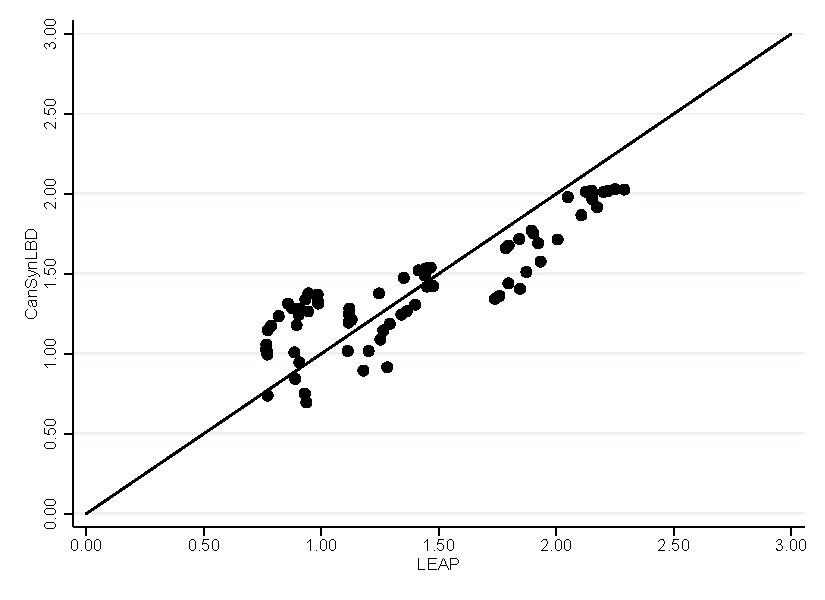
\includegraphics[trim=0 10 0 -20,clip,width=\linewidth]{graphs/Share_of_employment_by_NAICS_two-digit_and_year_Manufacturing_bw.pdf}
%\caption{CanSynLBD}
\end{subfigure}\\
\begin{subfigure}[h]{0.5\linewidth}
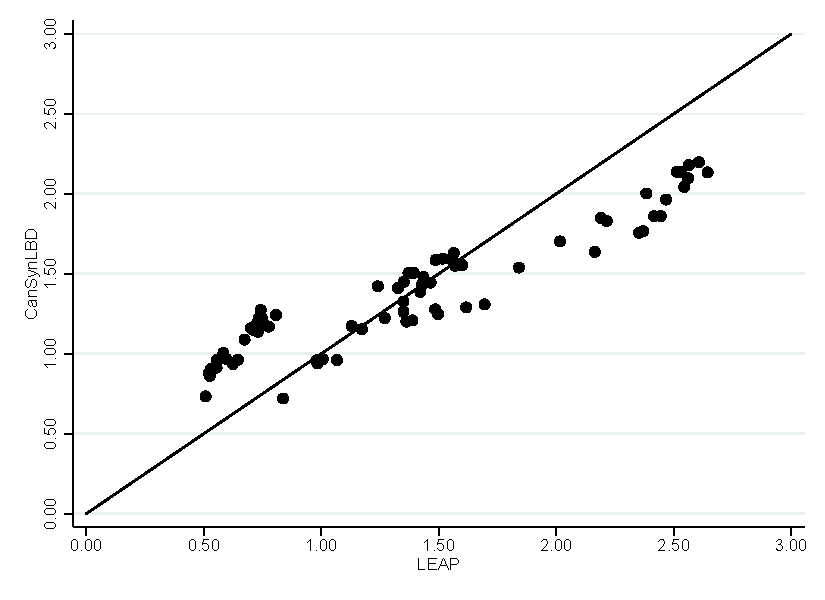
\includegraphics[trim=0 0 0 -20,clip,width=\linewidth]{graphs/Share_of_payroll_by_NAICS_two-digit_and_year_Manufacturing_bw.pdf}
\end{subfigure}
\caption{Share of entities (upper panel), share of employment (middle panel), and share of payroll (lower panel) by year and industry for the Canadian manufacturing sector.}\label{fig:FirmShare_manufac}
\end{figure}



%\begin{figure} [H]
%\centering
%\caption{Share of firms by NAICS two-digit and year (private)} \label{FirmSharePrivate}
%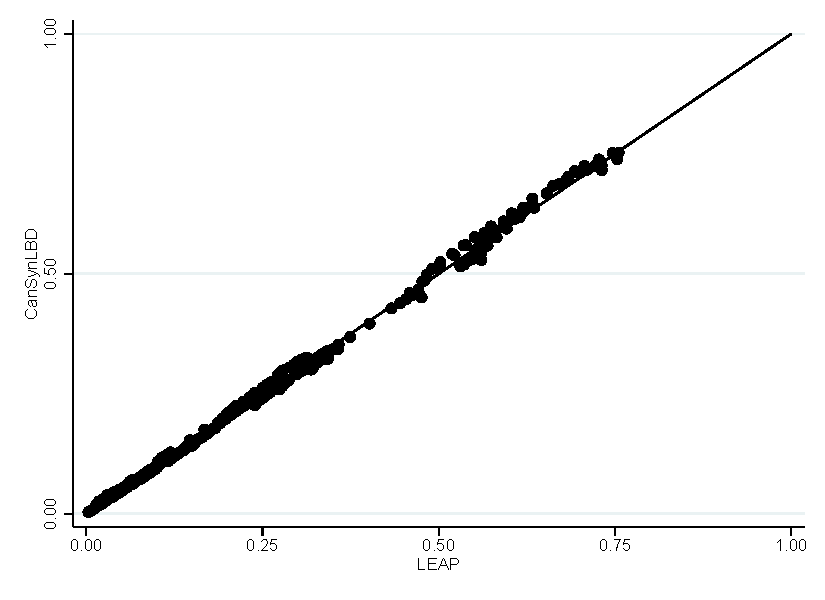
\includegraphics[height=2.8in, width=.7\linewidth]{graphs/Share_of_firms_by_NAICS_two-digit_and_year_private_bw.pdf} 
%\begin{minipage}{0.85\textwidth}
%{\footnotesize Note: \CanTableNote \par}
%\end{minipage}
%\end{figure}


%\vspace{-15.5pt}
%\begin{figure} [H]
%\centering
%\caption{Share of firms by NAICS two-digit and year (manufacturing)} \label{FirmShareManufacturing}
%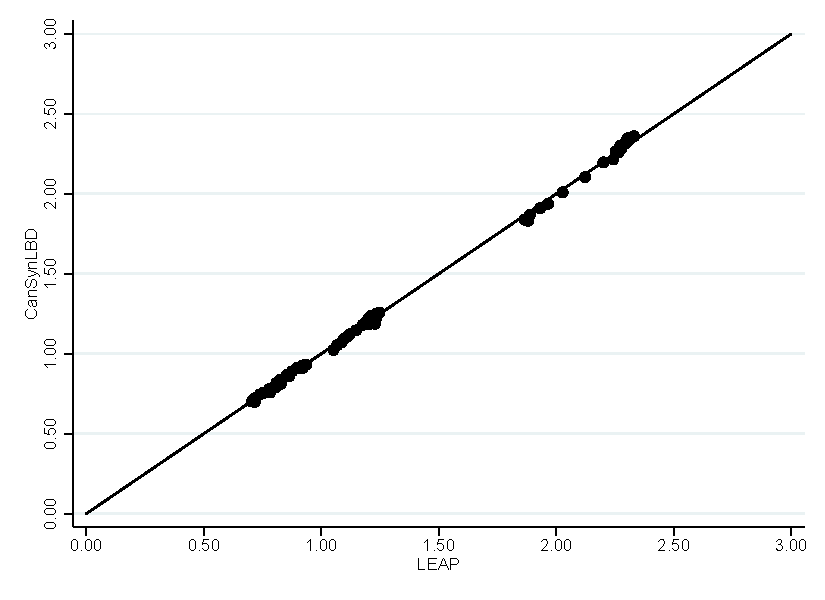
\includegraphics[height=2.8in, width=.7\linewidth]{graphs/Share_of_firms_by_NAICS_two-digit_and_year_Manufacturing_bw.pdf} 
%\begin{minipage}{0.85\textwidth}
%{\footnotesize Note: \CanTableNote \par}
%\end{minipage}
%\end{figure}



%\begin{figure} [H]
%\centering
%\caption{Share of employment by NAICS two-digit and year (private)} \label{EmploymentSharePrivate}
%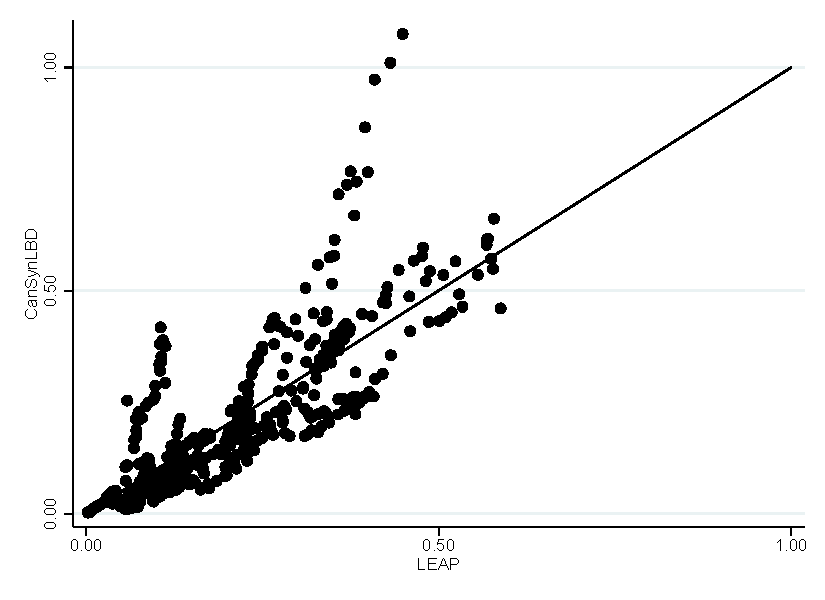
\includegraphics[height=2.8in, width=.7\linewidth]{graphs/Share_of_employment_by_NAICS_two-digit_and_year_private_bw.pdf} 
%\begin{minipage}{0.85\textwidth}
%{\footnotesize Note: \CanTableNote \par}
%\end{minipage}
%\end{figure}
%\vspace{-15.5pt}
%\begin{figure} [H]
%\centering
%\caption{Share of employment by NAICS two-digit and year (manufacturing)} \label{EmploymentShareManufacturing}
%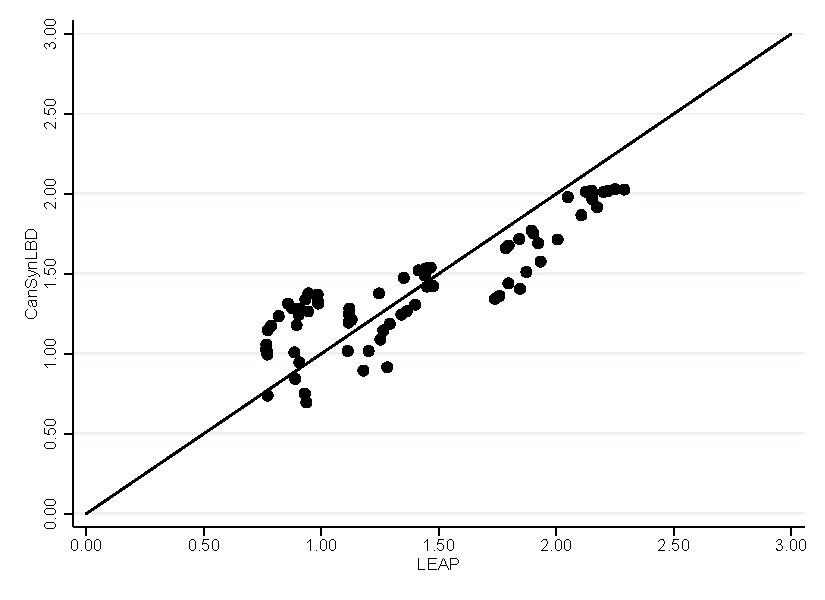
\includegraphics[height=2.8in, width=.7\linewidth]{graphs/Share_of_employment_by_NAICS_two-digit_and_year_Manufacturing_bw.pdf} 
%\begin{minipage}{0.85\textwidth}
%{\footnotesize Note: \CanTableNote \par}
%5\end{minipage}
%\end{figure}




%\begin{figure} [H]
%\centering
%\caption{Share of payroll by NAICS two-digit and year (private)} \label{PayrollSharePrivate}
%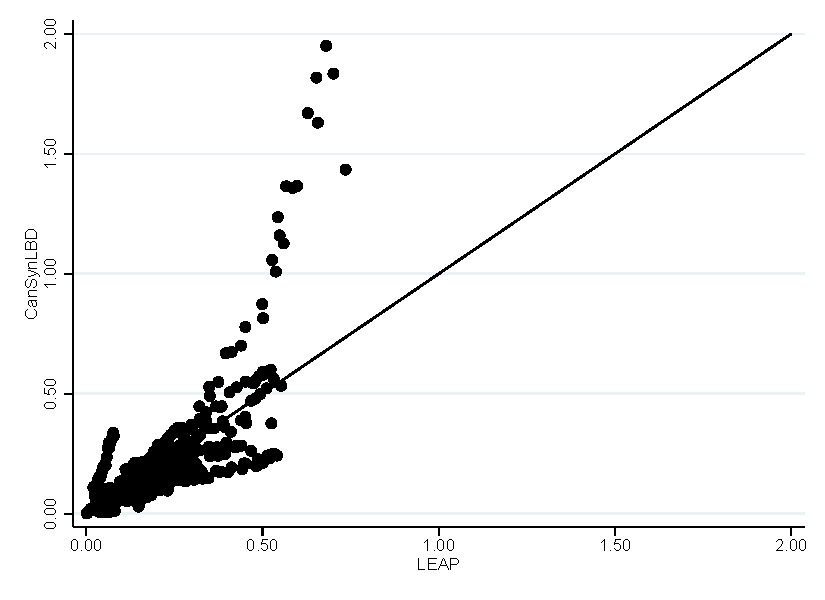
\includegraphics[height=2.8in, width=.7\linewidth]{graphs/Share_of_payroll_by_NAICS_two-digit_and_year_private_bw.pdf} 
%\begin{minipage}{0.85\textwidth}
%{\footnotesize Note: \CanTableNote \par}
%\end{minipage}
%\end{figure}
%\vspace{-15.5pt}
%\begin{figure} [H]
%\centering
%\caption{Share of payroll by NAICS two-digit and year (manufacturing)} \label{PayrollShareManufacturing}
%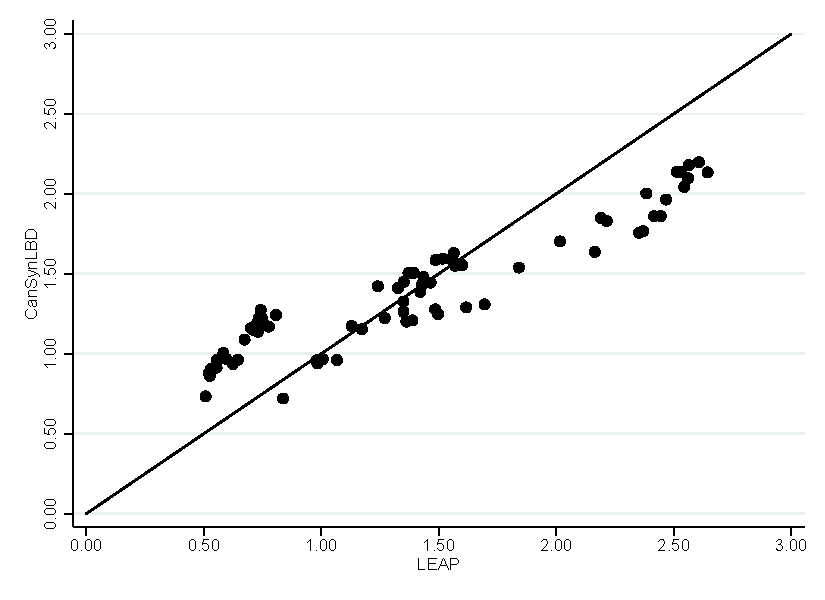
\includegraphics[height=2.8in, width=.7\linewidth]{graphs/Share_of_payroll_by_NAICS_two-digit_and_year_Manufacturing_bw.pdf} 
%\begin{minipage}{0.85\textwidth}
%{\footnotesize Note: \CanTableNote \par}
%\end{minipage}
%\end{figure}




















\section{Appendix Tables}
\label{sec:appendix_tables}

%\begin{table}[H]
%  \centering
%\begin{threeparttable}
% \caption{Entry and exit rates by year (LEAP)} \label{tab:Can:FirmDynamics} \medskip
%\renewcommand{\arraystretch}{1}
%\begin{tabular}{l|c c| c c| c c}
%\toprule
%&\multicolumn{2}{c|}{\textbf{LEAP}} &  \multicolumn{2}{c|}{\textbf{CanSynLBD}}&  \multicolumn{2}{c}{\textbf{Divergence}}\\
%\textbf{Year}&\textbf{Entry Rate}&\textbf{Exit Rate}&\textbf{Entry Rate}&\textbf{Exit Rate} &\textbf{Entry Rate}&\textbf{Exit Rate}\\
%\midrule
%1992&11.77&11.72&11.16&11.71&-0.60&-0.00\\
1993&11.81&11.61&10.84&12.18&-0.97&0.57\\
1994&12.04&11.79&11.57&12.01&-0.47&0.22\\
1995&11.94&12.09&11.69&12.26&-0.25&0.17\\
1996&12.91&10.31&12.62&10.64&-0.29&0.32\\
1997&13.18&9.75&13.03&10.21&-0.15&0.47\\
1998&12.48&10.89&12.97&10.13&0.50&-0.75\\
1999&12.00&10.66&12.16&9.97&0.16&-0.69\\
2000&11.80&10.51&11.59&9.70&-0.20&-0.82\\
2001&11.44&10.20&11.33&9.52&-0.12&-0.68\\
2002&11.39&9.91&11.10&9.03&-0.29&-0.89\\
2003&11.17&10.21&10.52&9.37&-0.65&-0.84\\
2004&12.13&9.76&10.94&9.57&-1.20&-0.20\\
2005&11.92&10.07&11.07&9.86&-0.84&-0.21\\
2006&11.81&9.96&11.15&9.34&-0.66&-0.62\\
2007&12.28&9.80&10.99&9.31&-1.29&-0.49\\
2008&11.60&10.14&10.78&9.75&-0.82&-0.40\\
2009&10.77&9.93&9.99&9.81&-0.78&-0.12\\
2010&10.80&9.75&9.91&9.65&-0.89&-0.10\\
2011&10.62&9.79&9.73&10.00&-0.89&0.21\\
2012&10.60&9.76&10.02&10.20&-0.58&0.44\\
2013&10.16&9.71&9.95&10.32&-0.21&0.62\\
2014&9.93&10.11&9.26&10.70&-0.67&0.59\\

%   \bottomrule
%  \end{tabular} 
%\begin{tablenotes}
%\small
%\item Note: \CanTableNote  We calculate the divergence of entry rate as the entry rate of CanSynLBD net of the entry rate of LEAP and the divergence of exit rate as the exit rate of CanSynLBD net of the exit rate of LEAP. Private sector only.
% \end{tablenotes}
% \end{threeparttable}
%\end{table}

%\begin{table}[H]
%  \centering
%\begin{threeparttable}
% \caption{Entry and exit rates by year (GLBD)} \label{tab:DE:FirmDynamics} \medskip
%\renewcommand{\arraystretch}{1}
%\begin{tabular}{l|c c| c c| c c}
%\toprule
%&\multicolumn{2}{c|}{\textbf{GLBD}} &  \multicolumn{2}{c|}{\textbf{GSynLBD}}&  \multicolumn{2}{c}{\textbf{Divergence}}\\
%\textbf{Year}&\textbf{Entry Rate}&\textbf{Exit Rate}&\textbf{Entry Rate}&\textbf{Exit Rate} &\textbf{Entry Rate}&\textbf{Exit Rate}\\
%\midrule
%1977&10.09&9.25&8.06&5.17&-2.03&-4.08\\
1978&10.81&9.22&7.97&5.40&-2.84&-3.81\\
1979&11.20&8.37&8.38&5.26&-2.81&-3.11\\
1980&10.85&8.77&7.74&5.40&-3.11&-3.37\\
1981&9.88&9.36&6.68&6.22&-3.20&-3.14\\
1982&9.15&9.63&6.48&5.83&-2.67&-3.80\\
1983&9.19&9.31&6.35&5.52&-2.84&-3.80\\
1984&10.51&8.58&7.10&5.08&-3.41&-3.50\\
1985&9.74&9.82&7.48&5.81&-2.26&-4.01\\
1986&12.01&9.08&8.04&5.34&-3.97&-3.74\\
1987&11.10&8.46&8.18&5.74&-2.92&-2.72\\
1988&11.15&9.51&7.64&5.36&-3.50&-4.15\\
1989&11.21&8.75&8.26&5.92&-2.95&-2.83\\
1990&13.11&9.00&10.44&5.85&-2.68&-3.15\\
1991&14.37&9.20&19.51&5.70&5.14&-3.50\\
1992&12.90&11.07&16.66&6.91&3.76&-4.17\\
1993&27.66&9.38&10.44&7.81&-17.23&-1.57\\
1994&13.13&11.68&10.34&7.54&-2.78&-4.14\\
1995&13.36&11.18&9.79&7.44&-3.57&-3.74\\
1996&12.15&11.39&8.46&7.46&-3.69&-3.93\\
1997&12.33&11.34&9.76&6.96&-2.57&-4.39\\
1998&14.59&11.30&10.58&7.34&-4.01&-3.96\\
1999&22.29&9.85&15.22&7.65&-7.07&-2.20\\
2000&12.92&11.52&9.07&9.42&-3.85&-2.10\\
2001&11.22&12.52&8.22&9.47&-3.00&-3.05\\
2002&10.63&12.99&7.41&8.93&-3.21&-4.06\\
2003&11.19&12.47&7.62&8.89&-3.57&-3.59\\
2004&11.54&10.71&7.82&7.95&-3.72&-2.76\\
2005&10.23&11.07&7.20&7.95&-3.03&-3.12\\
2006&10.23&10.25&7.28&7.15&-2.94&-3.10\\
2007&9.82&8.88&6.05&7.47&-3.77&-1.41\\
2008&8.73&9.61&5.93&8.24&-2.80&-1.37\\

%   \bottomrule
 % \end{tabular} 
%\begin{tablenotes}
%\small
%\item Note: We calculate the divergence of entry rate as the entry rate of GSynLBD net of the entry rate of GLBD and the divergence of exit rate as the exit rate of GSynLBD net of the exit rate of GLBD.
% \end{tablenotes}
% \end{threeparttable}
%\end{table}


\subsection{pMSE}
\label{sec:pmse_tables}

%%
%% Prior tables: logit and probit, uncorrected pMSE
%%

% \begin{table}[H]
%   \centering
%  \setlength{\tabcolsep}{11pt}
% \begin{threeparttable}
%  \caption{$pMSE$ estimates for CanSynLBD} \label{tab:pMSE_regression_can} \medskip
% \renewcommand{\arraystretch}{1}
% \begin{tabular}{l|c c| c c}
% \toprule
% \textbf{Independent Variables}&\multicolumn{2}{c|}{\textbf{Logistic Regression}} &  \multicolumn{2}{c}{\textbf{Probit Regression}}\\
% \midrule
%           &\multicolumn{1}{c}{Manufacturing}&\multicolumn{1}{c}{Private}&\multicolumn{1}{c}{Manufacturing}&\multicolumn{1}{c}{Private}\\
\hline
Ln ALU    &   0.1580\sym{***}&   0.7138\sym{***}&   0.1003\sym{***}&   0.4390\sym{***}\\
          & (0.0039)         & (0.0010)         & (0.0024)         & (0.0006)         \\
[1em]
Ln Pay    &   0.0039         &  -0.4426\sym{***}&   0.0012         &  -0.2691\sym{***}\\
          & (0.0037)         & (0.0010)         & (0.0023)         & (0.0006)         \\
[1em]
Age 3-4   &   0.0392\sym{***}&   0.0972\sym{***}&   0.0252\sym{***}&   0.0618\sym{***}\\
          & (0.0078)         & (0.0017)         & (0.0049)         & (0.0010)         \\
[1em]
Age 5-7   &  -0.0382\sym{***}&   0.0477\sym{***}&  -0.0233\sym{***}&   0.0309\sym{***}\\
          & (0.0073)         & (0.0016)         & (0.0045)         & (0.0010)         \\
[1em]
Age 8-12  &  -0.1258\sym{***}&  -0.0263\sym{***}&  -0.0781\sym{***}&  -0.0152\sym{***}\\
          & (0.0071)         & (0.0015)         & (0.0044)         & (0.0009)         \\
[1em]
Age 13 or more&  -0.2190\sym{***}&  -0.1024\sym{***}&  -0.1365\sym{***}&  -0.0627\sym{***}\\
          & (0.0074)         & (0.0016)         & (0.0046)         & (0.0010)         \\
\hline
\(N\)     &  2243011         & 34638723         &  2243011         & 34638723         \\
pseudo \(R^{2}\)&   0.0112         &   0.0318         &   0.0112         &   0.0320         \\
pMSE      &   0.0041         &   0.0121         &   0.0041         &   0.0124         \\

%   \bottomrule
%   \end{tabular} 
% \begin{tablenotes}
% \small
% \item \textit{Note}: An observation is a entity-year in the combined database. In all specifications, we include both time and industry fixed effects. Standard errors are in parentheses.  ***, **, and * indicate statistically significant coefficients at 1\%, 5\%, and 10\% percent levels, respectively.
%  \end{tablenotes}
%  \end{threeparttable}
% \end{table}

% \begin{table}[H]
%   \centering
% %\begin{threeparttable}
%  \caption{$pMSE$ estimates for GSynLBD} \label{tab:pMSE_regression_ger} \medskip
% \renewcommand{\arraystretch}{1}
% \begin{tabular}{l|c |c}
% \toprule
% \textbf{Independent Variables}&\textbf{Logistic Regression} &\textbf{Probit Regression}\\
% \midrule
% Ln ALU    &  -0.2895\sym{***}&  -0.1812\sym{***}\\
          & (0.0033)         & (0.0021)         \\
[1em]
Ln Pay    &   0.2584\sym{***}&   0.1618\sym{***}\\
          & (0.0028)         & (0.0018)         \\
[1em]
Age 3-4   &  -0.0987\sym{***}&  -0.0616\sym{***}\\
          & (0.0070)         & (0.0043)         \\
[1em]
Age 5-7   &  -0.0973\sym{***}&  -0.0608\sym{***}\\
          & (0.0066)         & (0.0041)         \\
[1em]
Age 8-12  &  -0.1172\sym{***}&  -0.0733\sym{***}\\
          & (0.0063)         & (0.0039)         \\
[1em]
Age 13 or more&  -0.1487\sym{***}&  -0.0930\sym{***}\\
          & (0.0059)         & (0.0037)         \\
\hline
\(N\)     &  2121956         &  2121956         \\
pseudo \(R^{2}\)&   0.0038         &   0.0038         \\
pMSE      &   0.0013         &   0.0013         \\

%   \bottomrule
%   \end{tabular} 
% \begin{tablenotes}
% \small
% \item \textit{Note}: An observation is a entity-year in the combined database. In all specifications, we include both time and industry fixed effects. Standard errors are in parentheses.  ***, **, and * indicate statistically significant coefficients at 1\%, 5\%, and 10\% percent levels, respectively.
%  \end{tablenotes}
% % \end{threeparttable}
% \end{table}

%%
%% After referee reports
%%


% Table created by stargazer v.5.2.2 by Marek Hlavac, Harvard University. E-mail: hlavac at fas.harvard.edu
% Date and time: Thu, Apr 30, 2020 - 05:35:47 PM
\begin{table}[!htbp] \centering 
\setlength{\tabcolsep}{11pt}
\begin{threeparttable}
  \caption{Detailed results for pMSE by sector and country} 
  \label{tab:pmse:details} 
\begin{tabular}{@{\extracolsep{5pt}} l|cc|c} 
\toprule
\textbf{Independent Variables} & \multicolumn{2}{c}{\textbf{Canada}} & \textbf{Germany}\\
\multicolumn{1}{r}{\it Sector:}&Manufacturing & Private & All \\ 
\midrule
Ln ALU & 0.158 & 0.7138 & -0.2895 \\ 
 & 0.0039 & 0.001 & 0.0033 \\ 
Ln Pay & 0.0039 & -0.4426 & 0.2584 \\ 
 & 0.0037 & 0.001 & 0.0028 \\ 
Age 3-4 & 0.0392 & 0.0972 & -0.0987 \\ 
 & 0.0078 & 0.0017 & 0.007 \\ 
Age 5-7 & -0.0382 & 0.0477 & -0.0973 \\ 
 & 0.0073 & 0.0016 & 0.0066 \\ 
Age 8-12 & -0.1258 & -0.0263 & -0.1172 \\ 
 & 0.0071 & 0.0015 & 0.0063 \\ 
Age 13 or more & -0.219 & -0.1024 & -0.1487 \\ 
 & 0.0074 & 0.0016 & 0.0059 \\ 
N & 2243011 & 34638723 & 2121956 \\ 
pseudo R-sq & 0.0112 & 0.0318 & 0.0038 \\ 
pMSE & 0.0041 & 0.0121 & 0.0013 \\ 
 & 0.0041 & 0.0121 & 0.0013 \\ 
\endrule
\end{tabular} 
\begin{tablenotes}
\small
\item \textit{Note}: An observation is a entity-year in the combined database. All specifications include  time and industry fixed effects. Standard errors are in parentheses. 
\end{tablenotes}
\end{threeparttable}
\end{table} 


\subsection{Regression analysis tables}
\label{sec:regression_tables}

\begin{table}[H]
  \centering
\begin{threeparttable}
 \caption{Regression coefficients (OLS) for LEAP} \label{tab:OLS_can} \medskip
\renewcommand{\arraystretch}{1}
\begin{tabular}{l|c c| c c}
\toprule
\textbf{Independent Variables}&\multicolumn{2}{c|}{\textbf{LEAP}} &  \multicolumn{2}{c}{\textbf{CanSynLBD}}\\
\midrule
&\multicolumn{1}{c}{Private}&\multicolumn{1}{c}{Manufacturing}&\multicolumn{1}{c}{Private}&\multicolumn{1}{c}{Manufacturing}\\
\hline
AR(1) Coefficient&   0.2031\sym{***}&   0.2481\sym{***}&   0.3970\sym{***}&   0.4405\sym{***}\\
          & (0.0001)         & (0.0005)         & (0.0002)         & (0.0007)         \\
[1em]
Ln Pay    &   0.7847\sym{***}&   0.7300\sym{***}&   0.5481\sym{***}&   0.5228\sym{***}\\
          & (0.0001)         & (0.0005)         & (0.0002)         & (0.0006)         \\
[1em]
Age 3-4   &  -0.1202\sym{***}&  -0.1717\sym{***}&  -0.1223\sym{***}&  -0.2340\sym{***}\\
          & (0.0003)         & (0.0014)         & (0.0004)         & (0.0016)         \\
[1em]
Age 5-7   &  -0.1260\sym{***}&  -0.1891\sym{***}&  -0.1235\sym{***}&  -0.2507\sym{***}\\
          & (0.0003)         & (0.0014)         & (0.0004)         & (0.0016)         \\
[1em]
Age 8-12  &  -0.1268\sym{***}&  -0.1973\sym{***}&  -0.1169\sym{***}&  -0.2551\sym{***}\\
          & (0.0003)         & (0.0013)         & (0.0004)         & (0.0016)         \\
[1em]
Age 13 or more&  -0.1246\sym{***}&  -0.1992\sym{***}&  -0.1101\sym{***}&  -0.2577\sym{***}\\
          & (0.0003)         & (0.0014)         & (0.0004)         & (0.0017)         \\
\hline
\(N\)     & 15708195         &  1015293         & 13573225         &   959764         \\
\(R^{2}\) &   0.9696         &   0.9743         &   0.9444         &   0.9523         \\

\bottomrule
\end{tabular} 
\begin{tablenotes}
\small
\item Note: In all specifications, we include both year and industry fixed effects. Standard errors are in parentheses.  ***, **, and * indicate statistically significant coefficients at 1\%, 5\%, and 10\% percent levels, respectively.
 \end{tablenotes}
 \end{threeparttable}
\end{table}

\begin{table}[H]
  \centering
%\begin{threeparttable}
 \caption{Regression coefficients (OLS) for GLBD} \label{tab:OLS_ger} \medskip
\renewcommand{\arraystretch}{1}
\setlength{\tabcolsep}{14pt}
\begin{tabular}{l|c |c}
\toprule
\textbf{Independent Variables}&\textbf{GLBD} &  \textbf{GSynLBD}\\
\midrule
\hline
AR(1) Coefficient&   0.4430\sym{***}&   0.4143\sym{***}\\
          & (0.0007)         & (0.0008)         \\
[1em]
Ln Pay    &   0.4629\sym{***}&   0.5143\sym{***}\\
          & (0.0006)         & (0.0007)         \\
[1em]
Age 3-4   &  -0.0695\sym{***}&  -0.0642\sym{***}\\
          & (0.0017)         & (0.0016)         \\
[1em]
Age 5-7   &  -0.1066\sym{***}&  -0.0891\sym{***}\\
          & (0.0017)         & (0.0016)         \\
[1em]
Age 8-12  &  -0.1324\sym{***}&  -0.1109\sym{***}\\
          & (0.0017)         & (0.0016)         \\
[1em]
Age 13 or more&  -0.1880\sym{***}&  -0.1600\sym{***}\\
          & (0.0016)         & (0.0015)         \\
\hline
\(N\)     &   848871         &   966084         \\
\(R^{2}\) &   0.9167         &   0.8968         \\

   \bottomrule
  \end{tabular} 
\begin{tablenotes}
\small
\item Note: In all specifications, we include both year and industry fixed effects. Standard errors are in parentheses.  ***, **, and * indicate statistically significant coefficients at 1\%, 5\%, and 10\% percent levels, respectively.
 \end{tablenotes}
 %\end{threeparttable}
\end{table}


%%%%%%%%%%%%%%%%%%%%%%%%%%% GMM

\begin{table}[H]
  \centering
\begin{threeparttable}
 \caption{Regression coefficients (Dynamic) for LEAP} \label{tab:Dynamic - GMM_can} \medskip
\renewcommand{\arraystretch}{1}
\begin{tabular}{l|c c| c c}
\toprule
\textbf{Independent Variables}&\multicolumn{2}{c|}{\textbf{LEAP}} &  \multicolumn{2}{c}{\textbf{CanSynLBD}}\\
\midrule
&\multicolumn{1}{c}{Private}&\multicolumn{1}{c}{Manufacturing}&\multicolumn{1}{c}{Private}&\multicolumn{1}{c}{Manufacturing}\\
\hline
AR(1) Coefficient&   0.0805\sym{***}&   0.1189\sym{***}&   0.5722\sym{***}&   0.5425\sym{***}\\
          & (0.0003)         & (0.0018)         & (0.0024)         & (0.0084)         \\
[1em]
Ln Pay    &   0.8991\sym{***}&   0.8523\sym{***}&   0.4101\sym{***}&   0.4302\sym{***}\\
          & (0.0002)         & (0.0015)         & (0.0018)         & (0.0067)         \\
[1em]
Age 3-4   &  -0.0450\sym{***}&  -0.0797\sym{***}&  -0.2075\sym{***}&  -0.2972\sym{***}\\
          & (0.0002)         & (0.0014)         & (0.0010)         & (0.0051)         \\
[1em]
Age 5-7   &  -0.0438\sym{***}&  -0.0860\sym{***}&  -0.2129\sym{***}&  -0.3162\sym{***}\\
          & (0.0002)         & (0.0015)         & (0.0011)         & (0.0059)         \\
[1em]
Age 8-12  &  -0.0418\sym{***}&  -0.0923\sym{***}&  -0.2187\sym{***}&  -0.3294\sym{***}\\
          & (0.0003)         & (0.0017)         & (0.0013)         & (0.0070)         \\
[1em]
Age 13 or more&  -0.0379\sym{***}&  -0.0898\sym{***}&  -0.2318\sym{***}&  -0.3414\sym{***}\\
          & (0.0003)         & (0.0019)         & (0.0015)         & (0.0080)         \\
\hline
\(N\)     & 15708195         &  1015293         & 13573225         &   959764         \\
m2        & -14.5000         &  -2.2200         & -27.5400         &  -9.4400         \\
Sargan test&  6.9e+04         &  4.6e+03         &  1.5e+04         &  1.5e+03         \\
df of Sargan Test& 252.0000         & 252.0000         & 252.0000         & 252.0000         \\
P value of Sargan test&   0.0000         &   0.0000         &   0.0000         &   0.0000         \\

   \bottomrule
  \end{tabular} 
\begin{tablenotes}
\small
\item Note: In this table, $m2$ is the Arellano-Bond test for zero autocorrelation in first-differenced errors for order two. Standard errors are in parentheses. ***, **, and * indicate statistically significant coefficients at 1\%, 5\%, and 10\% percent levels, respectively.
 \end{tablenotes}
 \end{threeparttable}
\end{table}

\begin{table}[H]
  \centering
%\begin{threeparttable}
 \caption{Regression coefficients (Dynamic) for GLBD} \label{tab:Dynamic - GMM_ger} \medskip
\renewcommand{\arraystretch}{1}
\setlength{\tabcolsep}{13pt}
\begin{tabular}{l|c |c}
\toprule
\textbf{Independent Variables}&\textbf{GLBD} &\textbf{GSynLBD}\\
\midrule
AR(1) Coefficient&   0.0489\sym{***}&   0.6999\sym{***}\\
          & (0.0051)         & (0.0057)         \\
[1em]
Ln Pay    &   0.7559\sym{***}&   0.2916\sym{***}\\
          & (0.0035)         & (0.0042)         \\
[1em]
Age 3-4   &  -0.0070\sym{***}&  -0.1026\sym{***}\\
          & (0.0012)         & (0.0015)         \\
[1em]
Age 5-7   &  -0.0233\sym{***}&  -0.1386\sym{***}\\
          & (0.0014)         & (0.0017)         \\
[1em]
Age 8-12  &  -0.0473\sym{***}&  -0.1694\sym{***}\\
          & (0.0015)         & (0.0018)         \\
[1em]
Age 13 or more&  -0.1084\sym{***}&  -0.2183\sym{***}\\
          & (0.0015)         & (0.0018)         \\
\hline
\(N\)     &   848871         &   966084         \\
m2        &  -2.5100         &  -4.1300         \\
Sargan test&  3.6e+03         &  2.0e+03         \\
df of Sargan Test& 495.0000         & 495.0000         \\
P value of Sargan test&   0.0000         &   0.0000         \\

   \bottomrule
  \end{tabular} 
\begin{tablenotes}
\small
\item Note: In this table, $m2$ is the Arellano-Bond test for zero autocorrelation in first-differenced errors for order two. Standard errors are in parentheses. ***, **, and * indicate statistically significant coefficients at 1\%, 5\%, and 10\% percent levels, respectively.
 \end{tablenotes}
% \end{threeparttable}
\end{table}


%%%%%%%%%%%%%%%%   Dynamic System GMM


\begin{table}[H]
  \centering
\begin{threeparttable}
 \caption{Regression coefficients (Dynamic - system GMM) for LEAP} \label{tab:Dynamic - system GMM_can} \medskip
\renewcommand{\arraystretch}{1}
\begin{tabular}{l|c c| c c}
\toprule
\textbf{Independent Variables}&\multicolumn{2}{c|}{\textbf{LEAP}} &  \multicolumn{2}{c}{\textbf{CanSynLBD}}\\
\midrule
&\multicolumn{1}{c}{Private}&\multicolumn{1}{c}{Manufacturing}&\multicolumn{1}{c}{Private}&\multicolumn{1}{c}{Manufacturing}\\
\hline
AR(1) Coefficient&   0.0978\sym{***}&   0.1614\sym{***}&   0.5111\sym{***}&   0.5780\sym{***}\\
          & (0.0002)         & (0.0014)         & (0.0008)         & (0.0041)         \\
[1em]
Ln Pay    &   0.8854\sym{***}&   0.8161\sym{***}&   0.4562\sym{***}&   0.4022\sym{***}\\
          & (0.0002)         & (0.0012)         & (0.0006)         & (0.0033)         \\
[1em]
Age 3-4   &  -0.0555\sym{***}&  -0.1097\sym{***}&  -0.1828\sym{***}&  -0.3177\sym{***}\\
          & (0.0002)         & (0.0012)         & (0.0004)         & (0.0028)         \\
[1em]
Age 5-7   &  -0.0558\sym{***}&  -0.1201\sym{***}&  -0.1860\sym{***}&  -0.3408\sym{***}\\
          & (0.0002)         & (0.0013)         & (0.0005)         & (0.0031)         \\
[1em]
Age 8-12  &  -0.0548\sym{***}&  -0.1298\sym{***}&  -0.1875\sym{***}&  -0.3583\sym{***}\\
          & (0.0002)         & (0.0014)         & (0.0005)         & (0.0036)         \\
[1em]
Age 13 or more&  -0.0524\sym{***}&  -0.1317\sym{***}&  -0.1943\sym{***}&  -0.3747\sym{***}\\
          & (0.0002)         & (0.0016)         & (0.0006)         & (0.0041)         \\
\hline
\(N\)     & 15708195         &  1015293         & 13573225         &   959764         \\
m2        & -11.4300         &   1.3900         & -41.6000         &  -7.6700         \\
Sargan test&  7.7e+04         &  6.3e+03         &  1.8e+04         &  1.7e+03         \\
df of Sargan Test& 274.0000         & 274.0000         & 274.0000         & 274.0000         \\
P value of Sargan test&   0.0000         &   0.0000         &   0.0000         &   0.0000         \\

   \bottomrule
  \end{tabular} 
\begin{tablenotes}
\small
\item Note: An observation is an entity-year. In this table, $m2$ is the Arellano-Bond test for zero autocorrelation in first-differenced errors for order two. Standard errors are in parentheses. ***, **, and * indicate statistically significant coefficients at 1\%, 5\%, and 10\% percent levels, respectively.
 \end{tablenotes}
 \end{threeparttable}
\end{table}

\begin{table}[H]
  \centering
%\begin{threeparttable}
 \caption{Regression coefficients (Dynamic - system GMM) for GLBD} \label{tab:Dynamic - system GMM_ger} \medskip
\renewcommand{\arraystretch}{1}
\setlength{\tabcolsep}{14pt}
\begin{tabular}{l|c| c}
\toprule
\textbf{Independent Variables}&\textbf{GLBD} &\textbf{GSynLBD}\\
\midrule
AR(1) Coefficient&   0.1883\sym{***}&   0.6140\sym{***}\\
          & (0.0021)         & (0.0027)         \\
[1em]
Ln Pay    &   0.6599\sym{***}&   0.3553\sym{***}\\
          & (0.0014)         & (0.0020)         \\
[1em]
Age 3-4   &  -0.0292\sym{***}&  -0.0934\sym{***}\\
          & (0.0011)         & (0.0013)         \\
[1em]
Age 5-7   &  -0.0512\sym{***}&  -0.1266\sym{***}\\
          & (0.0011)         & (0.0014)         \\
[1em]
Age 8-12  &  -0.0791\sym{***}&  -0.1545\sym{***}\\
          & (0.0011)         & (0.0015)         \\
[1em]
Age 13 or more&  -0.1400\sym{***}&  -0.2012\sym{***}\\
          & (0.0011)         & (0.0015)         \\
\hline
\(N\)     &   848871         &   966084         \\
m2        &  19.4900         &  -8.8300         \\
Sargan test&  4.5e+03         &  2.8e+03         \\
df of Sargan Test& 526.0000         & 526.0000         \\
P value of Sargan test&   0.0000         &   0.0000         \\

   \bottomrule
  \end{tabular} 
\begin{tablenotes}
\small
\item Note: An observation is an entity-year. In this table, $m2$ is the Arellano-Bond test for zero autocorrelation in first-differenced errors for order two. Standard errors are in parentheses. ***, **, and * indicate statistically significant coefficients at 1\%, 5\%, and 10\% percent levels, respectively.
 \end{tablenotes}
 %\end{threeparttable}
\end{table}







%%%%%%%%%%%%%%%% Dynamic System GMM MA


\begin{table}[H]
  \centering
\begin{threeparttable}
 \caption{Regression coefficients (Dynamic - system GMM with MA(1)) for LEAP} \label{tab:Dynamic - system GMM with MA(1)_can} \medskip
\renewcommand{\arraystretch}{1}
\begin{tabular}{l|c c| c c}
\toprule
\textbf{Independent Variables}&\multicolumn{2}{c|}{\textbf{LEAP}} &  \multicolumn{2}{c}{\textbf{CanSynLBD}}\\
\midrule
&\multicolumn{1}{c}{Private}&\multicolumn{1}{c}{Manufacturing}&\multicolumn{1}{c}{Private}&\multicolumn{1}{c}{Manufacturing}\\
\hline
AR(1) Coefficient&   0.2005\sym{***}&   0.2821\sym{***}&   0.4850\sym{***}&   0.5737\sym{***}\\
          & (0.0007)         & (0.0040)         & (0.0012)         & (0.0059)         \\
[1em]
Ln Pay    &   0.8044\sym{***}&   0.7135\sym{***}&   0.4760\sym{***}&   0.4056\sym{***}\\
          & (0.0005)         & (0.0034)         & (0.0009)         & (0.0046)         \\
[1em]
Age 3-4   &  -0.1245\sym{***}&  -0.2033\sym{***}&  -0.1716\sym{***}&  -0.3158\sym{***}\\
          & (0.0005)         & (0.0032)         & (0.0006)         & (0.0037)         \\
[1em]
Age 5-7   &  -0.1328\sym{***}&  -0.2264\sym{***}&  -0.1733\sym{***}&  -0.3389\sym{***}\\
          & (0.0005)         & (0.0035)         & (0.0006)         & (0.0043)         \\
[1em]
Age 8-12  &  -0.1383\sym{***}&  -0.2454\sym{***}&  -0.1731\sym{***}&  -0.3560\sym{***}\\
          & (0.0006)         & (0.0039)         & (0.0007)         & (0.0051)         \\
[1em]
Age 13 or more&  -0.1441\sym{***}&  -0.2586\sym{***}&  -0.1774\sym{***}&  -0.3717\sym{***}\\
          & (0.0006)         & (0.0042)         & (0.0008)         & (0.0058)         \\
\hline
\(N\)     & 15708195         &  1015293         & 13573225         &   959764         \\
m2        &   8.2000         &   7.0600         & -40.0300         &  -6.6400         \\
Sargan test&  2.8e+04         &  2.3e+03         &  1.7e+04         &  1.3e+03         \\
df of Sargan Test& 251.0000         & 251.0000         & 251.0000         & 251.0000         \\
P value of Sargan test&   0.0000         &   0.0000         &   0.0000         &   0.0000         \\

   \bottomrule
  \end{tabular} 
\begin{tablenotes}
\small
\item Note: An observation is a firm and a year. In this table, $m2$ is the Arellano-Bond test for zero autocorrelation in first-differenced errors for order two. $LEAP$ is the Longitudinal Employment Analysis Program and $CanSynLBD$ is the Canadian synthetic database based on LEAP. In this table, we use 2015 vintage of LEAP and drop last year observation of each firm. Standard errors are in parentheses. ***, **, and * indicate statistically significant coefficients at 1\%, 5\%, and 10\% percent levels, respectively.
 \end{tablenotes}
 \end{threeparttable}
\end{table}

\begin{table}[H]
  \centering
%\begin{threeparttable}
 \caption{Regression coefficients (Dynamic - system GMM with MA(1)) for GLBD} \label{tab:Dynamic - system GMM with MA(1)_ger} \medskip
\renewcommand{\arraystretch}{1}
\setlength{\tabcolsep}{14pt}
\begin{tabular}{l|c| c}
\toprule
\textbf{Independent Variables}&\textbf{GLBD} &\textbf{GSynLBD}\\
\midrule
AR(1) Coefficient&   0.3701\sym{***}&   0.5268\sym{***}\\
          & (0.0060)         & (0.0048)         \\
[1em]
Ln Pay    &   0.5349\sym{***}&   0.4202\sym{***}\\
          & (0.0041)         & (0.0036)         \\
[1em]
Age 3-4   &  -0.0594\sym{***}&  -0.0831\sym{***}\\
          & (0.0015)         & (0.0013)         \\
[1em]
Age 5-7   &  -0.0922\sym{***}&  -0.1105\sym{***}\\
          & (0.0018)         & (0.0015)         \\
[1em]
Age 8-12  &  -0.1252\sym{***}&  -0.1351\sym{***}\\
          & (0.0019)         & (0.0016)         \\
[1em]
Age 13 or more&  -0.1850\sym{***}&  -0.1802\sym{***}\\
          & (0.0019)         & (0.0017)         \\
\hline
\(N\)     &   848871         &   966084         \\
m2        &  19.0300         & -11.6900         \\
Sargan test&  3.1e+03         &  2.5e+03         \\
df of Sargan Test& 494.0000         & 494.0000         \\
P value of Sargan test&   0.0000         &   0.0000         \\

   \bottomrule
  \end{tabular} 
\begin{tablenotes}
\small
\item Note: An observation is a firm and a year. In this table, $m2$ is the Arellano-Bond test for zero autocorrelation in first-differenced errors for order two. Standard errors are in parentheses. ***, **, and * indicate statistically significant coefficients at 1\%, 5\%, and 10\% percent levels, respectively.
 \end{tablenotes}
% \end{threeparttable}
\end{table}


% \section{Analytical validity}

% \todo{I don't think we need this part.}
% \subsection{Confidence interval for gross employment and other measures}
% We compute the standard error for gross employment as follows. We consider gross employment $E$ to be the sum of firm employments $E_j$:

% \begin{equation}
% E = \sum_j E_j
% \end{equation}

% Average firm employment $\bar{E} = \frac{E}{N_j}$ is assumed to be normally distributed, with standard deviation $\sigma_{\bar{E}}$. We compare the synthetic and the confidential data for gross employment, including error bands.



%\subsection{Other models}
%
%Possible papers:
%
%\begin{itemize}
%%\item %\textcite{10.1257/aer.20141280} use the BDS to show the role of firm size in firm dynamics, but also had access to the Synthetic LBD.
%\item \textcite{NBERc0480} use a cross-country dataset to study average post-entry behavior of young firms. 
%\end{itemize}

%\bibliographystyle{apalike}
%\bibliography{paper}

\section{Canada: Synthesized Observations}
\label{sec:synth_obs}


\begin{table}[H]
  \centering
\begin{threeparttable}
  \caption{Synthesized observations}  \label{tab:Synthesized_observations} \medskip
  \renewcommand{\arraystretch}{1}
  \begin{tabular}{l  c c }
    \toprule
    \textbf{Category}&\textbf{\# of Observations (millions)}&\textbf{Percentage}\\
    \midrule
Synthesized&22.01&93.35\\
Not synthesized&1.57&6.65\\
Total&23.58&100.00\\

   \bottomrule
  \end{tabular} 
\begin{tablenotes}
\small
\item Note: Not synthesized industries are NAICS 4481,    4482,     4483,     4511,     4513,     4841,     4842, 5241, and 5242. These industries are not converging for each time of implementation We drop industries, from the synthesized industries, which have less than ten observations in a given year. We do not synthesize the public sector (NAICS 61, 62, and 91).
 \end{tablenotes}
 \end{threeparttable}
\end{table}


\section{Confidentiality assessment}
\label{sec:conf:appendix}


\begin{table}[H]
\centering\footnotesize
\caption{Observed entity births given synthetic births for LEAP.} \label{tab:Can:ProbabilityPrivate} \medskip
\renewcommand{\arraystretch}{1}
\begin{tabular}{c c| c c c}
\toprule
\multicolumn{2}{c|}{\textbf{First (Birth) Year}} &  \multicolumn{3}{c}{\textbf{\% of Births over NAICS}}\\
\textbf{Synthetic}&\textbf{Actual}&\textbf{Minimum}&\textbf{Mean}&\textbf{Maximum}\\
\midrule
1991&1991&0.00&27.69&83.02\\
1992&1992&0.00&3.37&11.11\\
1993&1993&0.00&3.79&33.33\\
1994&1994&0.00&3.73&33.33\\
1995&1995&0.00&3.86&20.00\\
1996&1996&0.00&4.25&33.33\\
1997&1997&0.00&4.10&16.94\\
1998&1998&0.00&4.41&25.00\\
1999&1999&0.00&4.23&33.33\\
2000&2000&0.00&3.41&25.00\\
2001&2001&0.00&2.73&22.22\\
2002&2002&0.00&2.65&25.00\\
2003&2003&0.00&2.22&10.00\\
2004&2004&0.00&2.60&17.86\\
2005&2005&0.00&2.71&20.00\\
2006&2006&0.00&2.83&50.00\\
2007&2007&0.00&2.90&33.33\\
2008&2008&0.00&2.38&20.00\\
2009&2009&0.00&2.47&50.00\\
2010&2010&0.00&2.12&33.33\\
2011&2011&0.00&2.65&50.00\\
2012&2012&0.00&2.41&20.00\\
2013&2013&0.00&2.48&25.00\\
2014&2014&0.00&2.23&20.00\\
2015&2015&0.00&2.15&33.33\\

\bottomrule
\end{tabular} 
\\
\justify
%Note:
\end{table}



\begin{table}[H]
\centering\footnotesize
\caption{Observed entity births given synthetic births (GLBD)} \label{tab:GLBD:Probability} \medskip
\renewcommand{\arraystretch}{1}
\begin{tabular}{c c| c c c}
\toprule
\multicolumn{2}{c|}{\textbf{Birth Year}} &  \multicolumn{3}{c}{\textbf{\% of Births over NAICS}}\\
\textbf{Synthetic}&\textbf{Actual}&\textbf{Minimum}&\textbf{Mean}&\textbf{Maximum}\\
\midrule
1976&1976&1.55&1.62&1.68\\
1977&1977&1.35&1.55&1.75\\
1978&1978&0.97&1.50&2.02\\
1979&1979&1.99&2.05&2.11\\
1980&1980&1.15&1.61&2.07\\
1981&1981&0.76&1.28&1.80\\
1982&1982&1.29&1.39&1.48\\
1983&1983&1.54&1.57&1.61\\
1984&1984&0.99&1.03&1.07\\
1985&1985&0.83&1.56&2.28\\
1986&1986&1.36&1.79&2.21\\
1987&1987&1.99&2.00&2.02\\
1988&1988&1.18&1.49&1.81\\
1989&1989&1.65&1.84&2.03\\
1990&1990&2.44&2.79&3.14\\
1991&1991&7.59&9.17&10.75\\
1992&1992&5.19&8.81&12.42\\
1993&1993&3.20&3.40&3.60\\
1994&1994&3.50&3.93&4.35\\
1995&1995&2.86&3.26&3.65\\
1996&1996&1.89&2.62&3.35\\
1997&1997&3.46&3.96&4.45\\
1998&1998&3.58&3.68&3.78\\
1999&1999&5.56&5.78&6.00\\
2000&2000&3.19&3.64&4.10\\
2001&2001&3.26&3.59&3.93\\
2002&2002&2.04&3.00&3.97\\
2003&2003&2.13&3.17&4.20\\
2004&2004&2.57&3.24&3.91\\
2005&2005&1.66&2.54&3.41\\
2006&2006&2.15&3.06&3.97\\
2007&2007&2.17&2.90&3.62\\
2008&2008&2.37&2.42&2.47\\
2009&2009&0.00&0.00&0.00\\
2010&2010&0.00&0.00&0.00\\

\bottomrule
\end{tabular} 
\\
\justify
%Note:
\end{table}

